\documentclass[a4paper,12pt]{article}

\usepackage[utf8]{inputenc}
\usepackage[english]{babel}
\usepackage{hyperref}
\usepackage{fontenc}
\usepackage{graphicx}
\usepackage{makeidx}
\usepackage{color}
\usepackage{multirow}
\usepackage{tabularx}
\usepackage{longtable}
\usepackage{url}
\usepackage{titlesec}
\usepackage{listings}
\usepackage{xcolor}
\usepackage{colortbl}
\usepackage{geometry}

\geometry{
    a4paper,
    left=25mm,
    right=25mm,
    top=30mm,
    bottom=30mm,
 }

%%%%%%%%%%%%%%%%%%%%%%%%%%%%%
%%%%%%% CONFIGURATION %%%%%%%
%%%%%%%%%%%%%%%%%%%%%%%%%%%%%
%%%%%%%%%%%%%%%%%%%%%%%%%%%%%%%%%%%%%%
%%%%%%% SECTION CONFIGURATIONS %%%%%%%
%%%%%%%%%%%%%%%%%%%%%%%%%%%%%%%%%%%%%%
\newcommand{\sectionbreak}{\clearpage}

\setcounter{secnumdepth}{5}

\titleformat{\paragraph}
{\normalfont\normalsize\bfseries}{\theparagraph}{1em}{}
\titlespacing*{\paragraph}
{0pt}{3.25ex plus 1ex minus .2ex}{1.5ex plus .2ex}


%%%%%%%%%%%%%%%%%%%%%%%%%%%%%%%%%%%%%%
%%%%%%% LISTINGS CONFIGURATION %%%%%%%
%%%%%%%%%%%%%%%%%%%%%%%%%%%%%%%%%%%%%%
\definecolor{mybg}{rgb}{1,1,0.8}
\definecolor{mysoftblue}{rgb}{0.6,0.729,0.867}
\definecolor{mygreen}{rgb}{0,0.6,0}
\definecolor{mygray}{rgb}{0.5,0.5,0.5}
\definecolor{mymauve}{rgb}{0.58,0,0.82}

\lstset{ %
  backgroundcolor=\color{mysoftblue},    % choose the background color; you must add \usepackage{color} or \usepackage{xcolor}
  basicstyle=\ttfamily\scriptsize,        % the size of the fonts that are used for the code
  breakatwhitespace=false,         % sets if automatic breaks should only happen at whitespace
  breaklines=true,                 % sets automatic line breaking
  captionpos=b,                    % sets the caption-position to bottom
  commentstyle=\color{mygreen},    % comment style
  deletekeywords={...},            % if you want to delete keywords from the given language
  escapeinside={\%*}{*)},          % if you want to add LaTeX within your code (example: \%* int v; *) )
  extendedchars=true,              % lets you use non-ASCII characters; for 8-bits encodings only, does not work with UTF-8
  frame=single,                    % adds a frame around the code (none, single)
  keepspaces=true,                 % keeps spaces in text, useful for keeping indentation of code (possibly needs columns=flexible)
  keywordstyle=\color{blue},       % keyword style
  language=Java,                   % the language of the code
  otherkeywords={*,...},           % if you want to add more keywords to the set
  numbers=none,                    % where to put the line-numbers; possible values are (none, left, right)
  numbersep=5pt,                   % how far the line-numbers are from the code
  numberstyle=\tiny\color{mygray}, % the style that is used for the line-numbers
  rulecolor=\color{black},         % if not set, the frame-color may be changed on line-breaks within not-black text (e.g. comments (green here))
  showspaces=false,                % show spaces everywhere adding particular underscores; it overrides 'showstringspaces'
  showstringspaces=false,          % underline spaces within strings only
  showtabs=false,                  % show tabs within strings adding particular underscores
  stepnumber=2,                    % the step between two line-numbers. If it's 1, each line will be numbered
  stringstyle=\color{mymauve},     % string literal style
  tabsize=2,                       % sets default tabsize to 2 spaces
  title=\lstname,                  % show the filename of files included with \lstinputlisting; also try caption instead of title
  aboveskip=20pt,                  % space left avobe the listing
  belowskip=0pt,                   % space left below the listing
  columns=fullflexible             % to allow automatic copy from listings
}


%%%%%%%%%%%%%%%%%%%%%%%%%%%%%%%%%%%
%%%%%%% OTHER CONFIGURATION %%%%%%%
%%%%%%%%%%%%%%%%%%%%%%%%%%%%%%%%%%%

% Horizontal line
\newcommand{\HRule}{
  \rule{\linewidth}{0.5mm}
}

% Color box for comments
\newcommand{\colorComment}[1]{
\begin{table}[h]
    \centering
    \begin{tabular}{p{0.8\textwidth}}
        \cellcolor{orange}\begin{center}
	  #1 \\
        \end{center}
        \\
    \end{tabular}
\end{table}
}
\title{COMP Superscalar}
\author{Installation Manual}
\date{Version 1.4}


%%%%%%%%%%%%%%%%%%%%%%%%%%%%%
%%%%%%%% DOCUMENT %%%%%%%%%%%
%%%%%%%%%%%%%%%%%%%%%%%%%%%%%
\begin{document}

  %%%%%%%%%%%% TITLE PAGE %%%%%%%%%%%%%
  \hypersetup{pageanchor=false}
  \begin{titlepage} 
    \begin{center} 
      
\includegraphics[width=0.3\textwidth]{./Figures/Logos/degradado-naranja-compss.jpg}~\\[1cm] 
      \textsc{\LARGE COMP Superscalar}\\[1.5cm] 
      
      \HRule \\[0.4cm] 
      { \huge \bfseries Installation Manual \\[0.4cm] }
      \HRule \\[1.5cm] 

      { \large \textsc{Version: 1.3 }} \\[0.3cm]
      { \large \today } 
      
      \vfill 
      % Bottom of the page
      
\includegraphics[width=0.5\textwidth]{./Figures/bsc_280.jpg}~\\[1cm]
    \end{center} 
  \end{titlepage}
  \hypersetup{pageanchor=true}
  
  %%%%%%%% REFERENCE NOTES %%%%%%%%%%
  {
    This manual only provides information about how to install and configure COMPSs. Specifically, it details the installation 
    process for Debian based distributions and for RedHat based distributions, and the steps to configure COMPSs properly.
    \newline
    
    If you are not wondering to install COMPSs please consider using our already prepared \textit{Virtual Machine} available
    at our webpage: \url{http://compss.bsc.es} .
    \newline
    
    For further information about the application execution please refer to the \textit{COMPSs User Manual: Application execution
    guide} available at \url{http://compss.bsc.es} .
    
    For further information about the application development please refer to the \textit{COMPSs User Manual: Application development
    guide} available at \url{http://compss.bsc.es/} .
    
    For full COMPSs application examples (codes, execution commands, results, logs, etc.) please refer to the \textit{COMPSs Sample 
    Applications} available at \url{http://compss.bsc.es/} .
  }
  
  %%%%%%%% TABLE OF CONTENTS %%%%%%%%%%
  \pagenumbering{roman}
  \setcounter{tocdepth}{6}
  \tableofcontents
  %\listoffigures
  %\listoftables
    
  \newpage

  %%%%%%%%%%%%% CONTENTS %%%%%%%%%%%%%%
  \pagenumbering{arabic}
    
  \section{COMP Superscalar (COMPSs)}
\label{sec:Introduction}

COMP Superscalar (COMPSs) is a programming model which aims to ease the development of applications for distributed infrastructures, such as Clusters, Grids and Clouds. COMP superscalar also features a runtime system that exploits the inherent parallelism of applications at execution time.

For the sake of programming productivity, the COMPSs model has four key characteristics:

\begin{itemize}
 
 \item  {\bf Sequential programming:} COMPSs programmers do not need to deal with the typical duties of parallelization and distribution, such as thread creation and synchronization, data distribution, messaging or fault tolerance. Instead, the model is based on sequential programming, which makes it appealing to users that either lack parallel programming expertise or are looking for better programmability.
 
 \item  {\bf Infrastructure unaware:} COMPSs offers a model that abstracts the application from the underlying distributed infrastructure. Hence, COMPSs programs do not include any detail that could tie them to a particular platform, like deployment or resource management. This makes applications portable between infrastructures with diverse characteristics.
 
 \item  {\bf Standard programming languages:} COMPSs is based on the popular programming language Java, but also offers language bindings for Python and C/C++ applications. This facilitates the learning of the model, since programmers can reuse most of their previous knowledge.
 
 \item  {\bf No APIs:} In the case of COMPSs applications in Java, the model does not require to use any special API call, pragma or construct in the application; everything is pure standard Java syntax and libraries. With regard the Python and C/C++ bindings, a small set of API calls should be used on the COMPSs applications.

\end{itemize}



  \section{Packages description}
\label{sec:Packages}


\subsection{Packages structure}
Despite the fact that we recomend users to install the complete COMPSs Framework, we have built different packages to allow users
customize as maximum as possible their installation. Figure \ref{fig:compss_packages_debian} illustrates the COMPSs 
packaging structure and its internal dependencies. 
\begin{figure}[ht!]
  \centering
    \includegraphics[width=0.75\textwidth]{./Sections/2_Packages_Description/Figures/compss_packages.jpeg}
    \caption{COMPSs packaging structure}
    \label{fig:compss_packages_debian}
\end{figure}

\newpage

\subsection{Packages Dependencies}
Next we provide a list of dependencies for each COMPSs package. The exact names may vary depending on 
the Linux distribution but this list provides a general overview of the COMPSs dependencies. For specific information about
your distribution please check the \textit{Depends} section at you package manager (apt, yum, zypper, etc.).

\bgroup
  \def\arraystretch{1.5}
  \begin{center}
    \begin{tabular}{ p{6cm} | p{10cm} }
    COMPSs Framework 		& compss-runtime, compss-bindings, compss-tools, compss-cloud \\ \hline 
    COMPSs Runtime 		& compss-engine, compss-worker \\ \hline  
    COMPSs Engine 		& openjdk-7-jre, graphviz, xdg-utils \\ \hline 
    COMPSs Worker 		& openjdk-7-jre \\ \hline 
    COMPSs Bindings 		& compss-bindings-common, compss-c-binding, compss-python-binding \\ \hline 
    COMPSs Bindings Common 	& compss-engine, openjdk-7-jre \\ \hline 
    COMPSs Python Binding 	& compss-bindings-common, python ($>= 2.7$), libpython2.7 \\ \hline 
    COMPSs C/C++ Binding 	& compss-binding-common, openjdk-7-jre, automake, libtool, libboost-serialization-dev, libboost-iostreams-dev \\ \hline 
    COMPSs Tools 		& compss-extrae, compss-monitor \\ \hline 
    COMPSs Extrae 		& compss-engine, openjdk-7-jre, libxml2 ($>= 2.5$), libxml2-dev ($>= 2.5$), gfortran \\ \hline 
    COMPSs Monitor 		& compss-engine, openjdk-7-jre \\ \hline 
    COMPSs Cloud 		& compss-engine, openjdk-7-jre    
    \end{tabular}
  \end{center}
\egroup
  
  \section{Debian-based distributions}
\label{sec:Debian}


\subsection{Prerequisites}
The commands described on the following sections require root privileges and Internet connection.

Once the installation process is finished, please log out and back in again to complete the installation. 

\subsection{Package Repository}
To add the package repository you can easily download our predefined lists by executing the following command:
\begin{lstlisting}[language=bash]
x86_64 :
   wget http://compss.bsc.es/releases/repofiles/repo_deb_x86-64.list -O /etc/apt/sources.list.d/compss-framework_x86-64.list
   
noarch :
   wget http://compss.bsc.es/releases/repofiles/repo_deb_noarch.list -O /etc/apt/sources.list.d/compss-framework_noarch.list
\end{lstlisting}

Next you need to add the repository key by executing:
\begin{lstlisting}[language=bash]
wget -qO - http://compss.bsc.es/repo/debs/deb-gpg-bsc-grid.pub.key | apt-key add -
\end{lstlisting}

And finally, refresh the apt-get repositories:
\begin{lstlisting}[language=bash]
apt-get update
\end{lstlisting}

\subsection{Installation}
Despite the fact that we recomend users to install the complete COMPSs Framework, we have built different packages to allow users
customize as maximum as possible their installation. Figure \ref{fig:compss_packages_debian} illustrates the COMPSs packaging structure.
\begin{figure}[ht!]
  \centering
    \includegraphics[width=0.75\textwidth]{./Sections/2_Debian/Figures/compss_packages.jpeg}
    \caption{COMPSs packaging structure}
    \label{fig:compss_packages_debian}
\end{figure}

\newpage
Next we describe the available packages and how to install them. 

\colorComment{If you are willing to have a full COMPSs installation just follow the COMPSs Framework instructions
and skip to next section.}

\begin{itemize}
 \item \textbf{COMPSs Framework} \newline
       Contains the all COMPSs functionalities including the Runtime, all the bindings, all the tools and the cloud connectors.
       \newline
       To install this package please run:
       \begin{lstlisting}[language=bash]
	  apt-get install compss-framework
       \end{lstlisting}
 \item \textbf{COMPSs Runtime} \newline
       Contains the COMPSs runtime to support the native functionalities. Install this package if you only need to support Java
       applications.
       \newline
       To install this package please run:
       \begin{lstlisting}[language=bash]
	  apt-get install compss-runtime
       \end{lstlisting}
       This package is composed of two sub-packages:
       \begin{itemize}
        \item \textbf{COMPSs Engine} \newline
	      Contains the COMPSs Engine, essential to run COMPSs applications as master.
	      \newline
	      To install this package please run:
	      \begin{lstlisting}[language=bash]
		  apt-get install compss-engine
	      \end{lstlisting}
        \item \textbf{COMPSs Worker} \newline
              Contains the minimum installation to allow any machine run as a COMPSs worker.
              \newline
              To install this package please run:
	      \begin{lstlisting}[language=bash]
		  apt-get install compss-worker
	      \end{lstlisting}
       \end{itemize}

 \item \textbf{COMPSs Bindings} \newline
       Contains all the bindings to support C/C++ and Python applications. 
       \newline
       To install this package please run:
       \begin{lstlisting}[language=bash]
	  apt-get install compss-bindings
       \end{lstlisting}
       This package is composed of three sub-packages:
       \begin{itemize}
        \item \textbf{COMPSs Bindings Common} \newline
	      Contains the API to allow any binding communicate with the COMPSs Runtime. It is necessary for any binding installation.
	      \newline
	      To install this package please run:
	      \begin{lstlisting}[language=bash]
		  apt-get install compss-bindings-common
	      \end{lstlisting}
        \item \textbf{COMPSs C/C++ Binding} \newline
	      Contains the C/C++ Binding
	      \newline
	      To install this package please run:
	      \begin{lstlisting}[language=bash]
		  apt-get install compss-c-binding
	      \end{lstlisting}
        \item \textbf{COMPSs Python Binding} \newline
	      Contains the Python Binding
	      \newline
	      To install this package please run:
	      \begin{lstlisting}[language=bash]
		  apt-get install compss-python-binding
	      \end{lstlisting}
       \end{itemize}

 \item \textbf{COMPSs Tools} \newline
       Contains all the COMPSs Tools.
       \newline
       To install this package please run:
       \begin{lstlisting}[language=bash]
	  apt-get install compss-tools
       \end{lstlisting}
       This package is composed of three sub-packages:
       \begin{itemize}
        \item \textbf{COMPSs Extrae} \newline
	      Contains the COMPSs Extrae tool needed to generate and process application traces.
	      \newline
	      To install this package please run:
	      \begin{lstlisting}[language=bash]
		  apt-get install compss-extrae
	      \end{lstlisting}
        \item \textbf{COMPSs Monitor} \newline
              Contains the COMPSs Monitor tool needed to monitor the application execution. 
              \newline
	      To install this package please run:
	      \begin{lstlisting}[language=bash]
		  apt-get install compss-monitor
	      \end{lstlisting}
       \end{itemize}

 \item \textbf{COMPSs Cloud} \newline
       Contains all the COMPSs Connectors needed to interact with the Cloud.
       \newline
       To install this package please run:
       \begin{lstlisting}[language=bash]
	  apt-get install compss-cloud
       \end{lstlisting}
\end{itemize} 

\subsection{Post installation}
Once your COMPSs package has been installed remember to log out and back in again to end the installation process.

If you need to setup your machine for the first time please take a look at Section \ref{sec:Additional_Configuration} for a 
detailed description of the additional configuration. 
          
  \section{RedHat-based distributions (zypper)}
\label{sec:RedHat_zypper}


\subsection{Prerequisites}
The commands described on the following sections require root privileges and Internet connection.

Once the installation process is finished, please log out and back in again to complete the installation. 

\subsection{Package Repository}
To add the package repository you can easily download our predefined lists by executing the following command:
\begin{lstlisting}[language=bash]
x86_64      :  zypper addrepo -f http://compss.bsc.es/repo/rpms/stable/suse/x86_64 compss
noarch      :  zypper addrepo -f http://compss.bsc.es/repo/rpms/stable/suse/noarch compss
\end{lstlisting}

And finally, refresh the apt-get repositories:
\begin{lstlisting}[language=bash]
zypper refresh
\end{lstlisting}

\subsection{Installation}
Despite the fact that we recomend users to install the complete COMPSs Framework, we have built different packages to allow users
customize as maximum as possible their installation. Next we describe the available packages and how to install them. 

\colorComment{If you are willing to have a full COMPSs installation just follow the COMPSs Framework instructions
and skip to next section.}

\begin{itemize}
 \item \textbf{COMPSs Framework} \newline
       Contains the all COMPSs functionalities including the Runtime, all the bindings, all the tools and the cloud connectors.
       \newline
       To install this package please run:
       \begin{lstlisting}[language=bash]
	  zypper install compss-framework
       \end{lstlisting}
 \item \textbf{COMPSs Runtime} \newline
       Contains the COMPSs runtime to support the native functionalities. Install this package if you only need to support Java
       applications.
       \newline
       To install this package please run:
       \begin{lstlisting}[language=bash]
	  zypper install compss-runtime
       \end{lstlisting}
       This package is composed of two sub-packages:
       \begin{itemize}
        \item \textbf{COMPSs Engine} \newline
	      Contains the COMPSs Engine, essential to run COMPSs applications as master.
	      \newline
	      To install this package please run:
	      \begin{lstlisting}[language=bash]
		  zypper install compss-engine
	      \end{lstlisting}
        \item \textbf{COMPSs Worker} \newline
              Contains the minimum installation to allow any machine run as a COMPSs worker.
              \newline
              To install this package please run:
	      \begin{lstlisting}[language=bash]
		  zypper install compss-worker
	      \end{lstlisting}
       \end{itemize}

 \item \textbf{COMPSs Bindings} \newline
       Contains all the bindings to support C/C++ and Python applications. 
       \newline
       To install this package please run:
       \begin{lstlisting}[language=bash]
	  zypper install compss-bindings
       \end{lstlisting}
       This package is composed of three sub-packages:
       \begin{itemize}
        \item \textbf{COMPSs Bindings Common} \newline
	      Contains the API to allow any binding communicate with the COMPSs Runtime. It is necessary for any binding installation.
	      \newline
	      To install this package please run:
	      \begin{lstlisting}[language=bash]
		  zypper install compss-bindings-common
	      \end{lstlisting}
        \item \textbf{COMPSs C/C++ Binding} \newline
	      Contains the C/C++ Binding
	      \newline
	      To install this package please run:
	      \begin{lstlisting}[language=bash]
		  zypper install compss-c-binding
	      \end{lstlisting}
        \item \textbf{COMPSs Python Binding} \newline
	      Contains the Python Binding
	      \newline
	      To install this package please run:
	      \begin{lstlisting}[language=bash]
		  zypper install compss-python-binding
	      \end{lstlisting}
       \end{itemize}

 \item \textbf{COMPSs Tools} \newline
       Contains all the COMPSs Tools.
       \newline
       To install this package please run:
       \begin{lstlisting}[language=bash]
	  zypper install compss-tools
       \end{lstlisting}
       This package is composed of three sub-packages:
       \begin{itemize}
        \item \textbf{COMPSs Extrae} \newline
	      Contains the COMPSs Extrae tool needed to generate and process application traces.
	      \newline
	      To install this package please run:
	      \begin{lstlisting}[language=bash]
		  zypper install compss-extrae
	      \end{lstlisting}
        \item \textbf{COMPSs Monitor} \newline
              Contains the COMPSs Monitor tool needed to monitor the application execution. 
              \newline
	      To install this package please run:
	      \begin{lstlisting}[language=bash]
		  zypper install compss-monitor
	      \end{lstlisting}
       \end{itemize}

 \item \textbf{COMPSs Cloud} \newline
       Contains all the COMPSs Connectors needed to interact with the Cloud.
       \newline
       To install this package please run:
       \begin{lstlisting}[language=bash]
	  zypper install compss-cloud
       \end{lstlisting}
\end{itemize} 

\subsection{Post installation}
Once your COMPSs package has been installed remember to log out and back in again to end the installation process.

If you need to setup your machine for the first time please take a look at Section \ref{sec:Additional_Configuration} for a 
detailed description of the additional configuration. 
  
  \section{RedHat-based distributions (yum)}
\label{sec:RedHat_yum}


\subsection{Prerequisites}
The commands described on the following sections require root privileges and Internet connection.

Once the installation process is finished, please log out and back in again to complete the installation. 

\subsection{Package Repository}
To add the package repository you can easily download our predefined lists by executing the following command:
\begin{lstlisting}[language=bash]
x86_64 :  
   wget http://compss.bsc.es/releases/repofiles/repo_rpm_centos_x86-64.repo -O /etc/yum.repos.d/compss-framework_x86-64.repo
   
noarch :
   wget http://compss.bsc.es/releases/repofile/repo_rpm_centos_noarch.repo -O /etc/yum.repos.d/compss-framework_noarch.repo
\end{lstlisting}


\subsection{Installation}
Despite the fact that we recomend users to install the complete COMPSs Framework, we have built different packages to allow users
customize as maximum as possible their installation. Figure \ref{fig:compss_packages_yum} illustrates the COMPSs packaging structure.
\begin{figure}[ht!]
  \centering
    \includegraphics[width=0.75\textwidth]{./Sections/4_RedHat_yum/Figures/compss_packages.jpeg}
    \caption{COMPSs Packaging structure}
    \label{fig:compss_packages_yum}
\end{figure}

\newpage
Next we describe the available packages and how to install them. 

\colorComment{If you are willing to have a full COMPSs installation just follow the COMPSs Framework instructions
and skip to next section.}

\begin{itemize}
 \item \textbf{COMPSs Framework} \newline
       Contains the all COMPSs functionalities including the Runtime, all the bindings, all the tools and the cloud connectors.
       \newline
       To install this package please run:
       \begin{lstlisting}[language=bash]
	  yum install compss-framework
       \end{lstlisting}
 \item \textbf{COMPSs Runtime} \newline
       Contains the COMPSs runtime to support the native functionalities. Install this package if you only need to support Java
       applications.
       \newline
       To install this package please run:
       \begin{lstlisting}[language=bash]
	  yum install compss-runtime
       \end{lstlisting}
       This package is composed of two sub-packages:
       \begin{itemize}
        \item \textbf{COMPSs Engine} \newline
	      Contains the COMPSs Engine, essential to run COMPSs applications as master.
	      \newline
	      To install this package please run:
	      \begin{lstlisting}[language=bash]
		  yum install compss-engine
	      \end{lstlisting}
        \item \textbf{COMPSs Worker} \newline
              Contains the minimum installation to allow any machine run as a COMPSs worker.
              \newline
              To install this package please run:
	      \begin{lstlisting}[language=bash]
		  yum install compss-worker
	      \end{lstlisting}
       \end{itemize}

 \item \textbf{COMPSs Bindings} \newline
       Contains all the bindings to support C/C++ and Python applications. 
       \newline
       To install this package please run:
       \begin{lstlisting}[language=bash]
	  yum install compss-bindings
       \end{lstlisting}
       This package is composed of three sub-packages:
       \begin{itemize}
        \item \textbf{COMPSs Bindings Common} \newline
	      Contains the API to allow any binding communicate with the COMPSs Runtime. It is necessary for any binding installation.
	      \newline
	      To install this package please run:
	      \begin{lstlisting}[language=bash]
		  yum install compss-bindings-common
	      \end{lstlisting}
        \item \textbf{COMPSs C/C++ Binding} \newline
	      Contains the C/C++ Binding
	      \newline
	      To install this package please run:
	      \begin{lstlisting}[language=bash]
		  yum install compss-c-binding
	      \end{lstlisting}
        \item \textbf{COMPSs Python Binding} \newline
	      Contains the Python Binding
	      \newline
	      To install this package please run:
	      \begin{lstlisting}[language=bash]
		  yum install compss-python-binding
	      \end{lstlisting}
       \end{itemize}

 \item \textbf{COMPSs Tools} \newline
       Contains all the COMPSs Tools.
       \newline
       To install this package please run:
       \begin{lstlisting}[language=bash]
	  yum install compss-tools
       \end{lstlisting}
       This package is composed of three sub-packages:
       \begin{itemize}
        \item \textbf{COMPSs Extrae} \newline
	      Contains the COMPSs Extrae tool needed to generate and process application traces.
	      \newline
	      To install this package please run:
	      \begin{lstlisting}[language=bash]
		  yum install compss-extrae
	      \end{lstlisting}
        \item \textbf{COMPSs Monitor} \newline
              Contains the COMPSs Monitor tool needed to monitor the application execution. 
              \newline
	      To install this package please run:
	      \begin{lstlisting}[language=bash]
		  yum install compss-monitor
	      \end{lstlisting}
       \end{itemize}

 \item \textbf{COMPSs Cloud} \newline
       Contains all the COMPSs Connectors needed to interact with the Cloud.
       \newline
       To install this package please run:
       \begin{lstlisting}[language=bash]
	  yum install compss-cloud
       \end{lstlisting}
\end{itemize} 

\subsection{Post installation}
Once your COMPSs package has been installed remember to log out and back in again to end the installation process.

If you need to setup your machine for the first time please take a look at Section \ref{sec:Additional_Configuration} for a 
detailed description of the additional configuration. 
  
  \section{Supercomputers}
\label{sec:Supercomputers}

The COMPSs Framework can be installed in any Supercomputer by installing its packages as in a normal distribution. The packages are
ready to be reallocated so the administrators can choose the right location for the COMPSs installation. \newline

However, if the administrators are not willing to install COMPSs through the packaging system, we also provide a \textbf{COMPSs 
zipped file} containing a pre-build script to easily install COMPSs. Next subsections provide further information about this process.

\subsection{Prerequisites}
In order to successfully run the installation script some dependencies must be present on the target machine. Administrators must 
provide the correct installation and environment of the following software:
\begin{itemize}
 \item Autotools
 \item BOOST
 \item Java 7 JRE
\end{itemize}

The following environment variables must be defined:
\begin{itemize}
 \item $JAVA\_HOME$
 \item $BOOST\_CPPFLAGS$
\end{itemize}

\subsection{Installation}
To perform the COMPSs Framework installation please execute the following commands:
\begin{lstlisting}[language=bash]
 # Check out the last COMPSs release
 $ wget http://compss.bsc.es/repo/sc/stable/COMPSs_1.3.tar.gz

 # Unpackage COMPSs
 $ tar -xvzf COMPSs_1.3.tar.gz
 
 # Install COMPSs at your preferred target location
 $ cd COMPSs
 $ ./install <targetDir>
 
 # Clean downloaded files
 $ rm -r COMPSs
 $ rm COMPSs_1.3.tar.gz
\end{lstlisting}

The installation script will create a COMPSs folder inside the given $<targetDir>$ so the final COMPSs installation will be placed 
under the $<targetDir>/COMPSs$ folder. Please note that if the folder already exists it will be \textbf{automatically erased}.

~ \newline
After completing the previous steps, administrators must ensure that the nodes have passwordless ssh access. If it is not the case,
please contact the COMPSs team at $support-compss@bsc.es$.

~ \newline
The COMPSs package also provides a \textit{compssenv} file that loads the required environment to allow users work more easily
with COMPSs. Thus, after the installation process we recomend to source the $<targetDir>/COMPSs/compssenv$ into the 
users \textit{.bashrc}.

~ \newline
Once done, remember to log out and back in again to end the installation process.

\subsection{Post installation}
To check that COMPSs Framework has been successfully installed you may run:
\begin{lstlisting}[language=bash]
 # Check the COMPSs version
 $ runcompss -v
 COMPSs version 1.3
\end{lstlisting}

For queue system executions, COMPSs provides several prebuild queue scripts than can be accessible throgh the \textit{enqueue\_compss}
command. Users can check the available options by running:
\begin{lstlisting}[language=bash]
$ enqueue_compss --help
Usage: /apps/COMPSs/1.3/Runtime/scripts/user/enqueue_compss 
         [queue_system_options] [COMPSs_options] 
         application_name application_arguments

* Options:
  General:
    --help, -h                              Print this help message
  
  Queue system configuration:
    - -exec_time=<minutes>                  Expected execution time of 
                                            the application (in minutes)
                                            Default: 10
                                            
    - -num_nodes=<int>                      Number of nodes to use
                                            Default: 2
                                            
    - -num_switches=<int>                   Maximum number of different switches.
                                            Select 0 for no restrictions.
                                            Maximum nodes per switch: 18
                                            Only available for at least 4 nodes. 
                                            Default: 0 
                                            
    - -queue_system=<name>                  Queue system to use: lsf | pbs | slurm
                                            Default: lsf
    - -queue=<name>                         Queue name to submit the job. 
                                            Depends on the queue system.
                                            For example (MN3): bsc_cs | bsc_debug
                                                | debug | interactive
                                            Default: default
                                            
    - -job_dependency=<jobID>               Postpone job execution until the job
                                            dependency has ended.
                                            Default: None
                                            
    - -tasks_per_node=<int>                 Maximum number of simultaneous
                                            tasks running on a node
                                            Default: 16
                                            
    - -master_working_dir=<path>            Working directory of the application
                                            Default: .
                                            
    - -worker_working_dir=<name>            Worker directory. Use: scratch | gpfs
                                            Default: scratch
                                            
    - -tasks_in_master=<int>                Maximum number of tasks that the master
                                            node can run as worker. Cannot exceed 
                                            tasks_per_node.
                                            Default: 0
                                            
    - -network=<name>                       Communication network for transfers:
                                            default | ethernet | infiniband | data.
                                            Default: infiniband
          
          
  Runcompss delegated parameters:

  Tools enablers:
    - -graph=<bool>, - -graph, -g           Generation of the complete graph (true/false)
                                            When no value is provided it is set to true
                                            Default: false
                                            
    - -tracing=<bool>, - -tracing, -t       Generation of traces (true/false)
                                            When no value is provided it is set to true
                                            Default: false
                                            
    - -monitoring=<int>, - -monitoring, -m  Period between monitoring samples 
                                            (milliseconds)
                                            When no value is provided it is set to 2000
                                            Default: 0
                                            
  Runtime configuration options:
    - -project=<path>                       Path to the project XML file
                                            Default: /gpfs/apps/MN3/COMPSs/1.3/Runtime/
                                            configuration/xml/projects/project.xml
                                            
    - -resources=<path>                     Path to the resources XML file
                                            Default: /gpfs/apps/MN3/COMPSs/1.3/Runtime/
                                            configuration/xml/resources/resources.xml
                                            
    - -lang=<name>                          Language of the application (java/c/python)
                                            Default: java
                                            
    - -log_level=<level>, - -debug, -d      Set the debug level: off | info | debug
                                            Default: off
  Advanced options:
    - -comm=<path>                          Class that implements the adaptor 
                                            for communications
                                            Supported adaptors: 
                                            integratedtoolkit.nio.master.NIOAdaptor | 
                                            integratedtoolkit.gat.master.GATAdaptor
                                            Default: 
                                              integratedtoolkit.nio.master.NIOAdaptor
                                              
    - -library_path=<path>                  Non-standard directories to search 
                                            for libraries (e.g. Java JVM library, 
                                            Python library, C binding library) 
                                            Default: Working Directory
                                            
    - -classpath=<path>                     Path for the application classes / modules
                                            Default: Working Directory
                                            
    - -task_count=<int>                     Only for C/Python Bindings. Maximum number
                                            of different functions/methods, invoked
                                            from the application, that have been
                                            selected as tasks
                                            Default: 50
                                            
    - -uuid=<int>                           Preset an application UUID
                                            Default: Automatic random generation
                                            
    - -PyObject_conversion=<bool>           Only for Python Binding. Enable the object
                                            conversion to string when possible
                                            (true/false).
                                            Default: false
                                            
* Application name:
    For Java applications:   Fully qualified name of the application
    For C applications:      Path to the master binary
    For Python applications: Path to the .py file containing the main program
    
* Application arguments:
    Command line arguments to pass to the application. Can be empty. 
                                            
\end{lstlisting}

If none of the pre-build sub-queue scripts adapts to your infrastructure (lsf, pbs, slurm, etc.) please contact 
the COMPSs team at $support-compss@bsc.es$ to find out a solution.

~ \newline
If you are willing to test the COMPSs Framework installation you can run any of the applications available at our application 
repository \url{https://compss.bsc.es/projects/bar}. We suggest to run the java simple application following the steps listed
inside its \textit{README} file. 

~ \newline
For further information about either the installation or the usage please check the \textit{README} file inside the COMPSs package. 


           
  \section{Additional Configuration}
\label{sec:Additional_Configuration}


\subsection{Configure SSH passwordless}
\label{subsec:Passwordless_ssh}
By default, COMPSs uses SSH libraries for communication between nodes. Consequently, after COMPSs is installed on a set of machines,
the SSH keys must be configured on those machines so that COMPSs can establish passwordless connections between them. This requires
to install the OpenSSH package (if not present already) and follow these steps \textbf{in each machine}:
\begin{enumerate}
 \item Generate an SSH key pair
       \begin{lstlisting}[language=bash]
	  $ ssh-keygen -t dsa
       \end{lstlisting}
 \item Distribute the public key to all the other machines and configure it as authorized
       \begin{lstlisting}[language=bash]
          For every other available machine (MACHINE):
	  $ scp ~/.ssh/id_dsa.pub MACHINE:./myDSA.pub
	  $ ssh MACHINE "cat ./myDSA.pub >> ~/.ssh/authorized_keys; rm ./myDSA.pub"
       \end{lstlisting}
 \item Check that passwordless SSH connections are working fine
       \begin{lstlisting}[language=bash]
          For every other available machine (MACHINE):
	  $ ssh MACHINE
       \end{lstlisting}
\end{enumerate}

For example, considering the cluster shown in Figure \ref{fig:cluster}, users will have to execute the following commands
to grant free ssh access between any pair of machines:
\begin{lstlisting}[language=bash]
 me@localhost:~$ ssh-keygen -t id_dsa
 # Granting access localhost -> m1.bsc.es
 me@localhost:~$ scp ~/.ssh/id_dsa.pub user_m1@m1.bsc.es:./me_localhost.pub
 me@localhost:~$ ssh user_m1@m1.bsc.es "cat ./me_localhost.pub >> ~/.ssh/authorized_keys; rm ./me_localhost.pub"
 # Granting access localhost -> m2.bsc.es
 me@localhost:~$ scp ~/.ssh/id_dsa.pub user_m2@m2.bsc.es:./me_localhost.pub
 me@localhost:~$ ssh user_m2@m2.bsc.es "cat ./me_localhost.pub >> ~/.ssh/authorized_keys; rm ./me_localhost.pub"
 
 me@localhost:~$ ssh user_m1@m1.bsc.es
 user_m1@m1.bsc.es:~> ssh-keygen -t id_dsa
 user_m1@m1.bsc.es:~> exit
 # Granting access m1.bsc.es -> localhost
 me@localhost:~$ scp user_m1@m1.bsc.es:~/.ssh/id_dsa.pub ~/userm1_m1.pub
 me@localhost:~$ cat ~/userm1_m1.pub >> ~/.ssh/authorized_keys
 # Granting access m1.bsc.es -> m2.bsc.es
 me@localhost:~$ scp ~/userm1_m1.pub user_m2@m2.bsc.es:~/userm1_m1.pub 
 me@localhost:~$ ssh user_m2@m2.bsc.es "cat ./userm1_m1.pub >> ~/.ssh/authorized_keys; rm ./userm1_m1.pub"
 me@localhost:~$ rm ~/userm1_m1.pub
 
 me@localhost:~$ ssh user_m2@m2.bsc.es
 user_m2@m2.bsc.es:~> ssh-keygen -t id_dsa
 user_m2@m2.bsc.es:~> exit
 # Granting access m2.bsc.es -> localhost
 me@localhost:~$ scp user_m2@m1.bsc.es:~/.ssh/id_dsa.pub ~/userm2_m2.pub
 me@localhost:~$ cat ~/userm2_m2.pub >> ~/.ssh/authorized_keys
 # Granting access m2.bsc.es -> m1.bsc.es
 me@localhost:~$ scp ~/userm2_m2.pub user_m1@m1.bsc.es:~/userm2_m2.pub 
 me@localhost:~$ ssh user_m1@m1.bsc.es "cat ./userm2_m2.pub >> ~/.ssh/authorized_keys; rm ./userm2_m2.pub"
 me@localhost:~$ rm ~/userm2_m2.pub
\end{lstlisting}

\begin{figure}[h!]
  \centering
    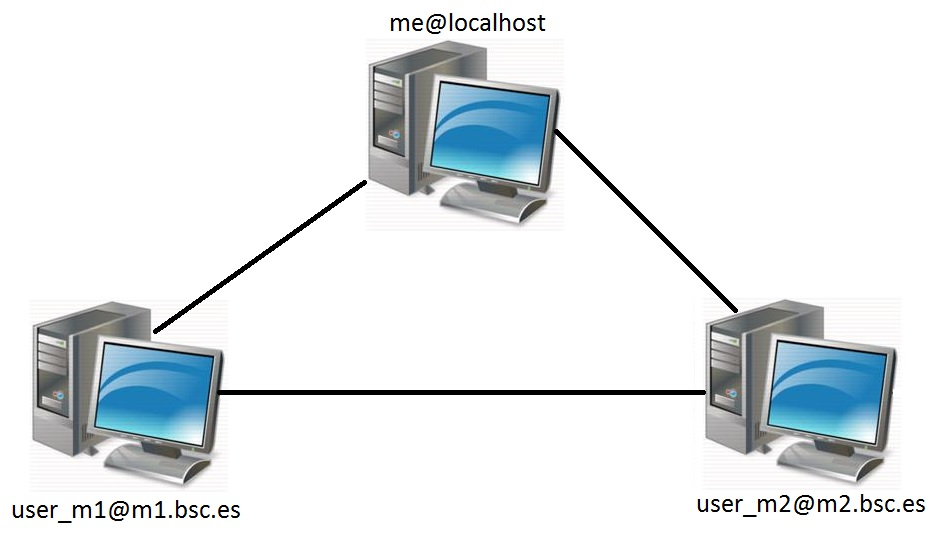
\includegraphics[width=0.95\textwidth]{./Sections/08_Additional_Configuration/Figures/cluster.jpeg}
    \caption{Cluster example}
    \label{fig:cluster}
\end{figure}


\subsection{Configure the COMPSs Cloud Connectors}
This section provides information about the additional configuration needed for some Cloud Connectors.

\subsubsection{OCCI (Open Cloud Computing Interface) connector}
In order to execute a COMPSs application using cloud resources, the rOCCI (Ruby OCCI) connector has to be configured properly.
The connector uses the rOCCI CLI client (upper versions from 4.2.5) which has to be installed in the node where the COMPSs main
application runs. The client can be installed following the instructions detailed at 
\url{http://appdb.egi.eu/store/software/rocci.cli}
  
  \section{COMPSs Removal}
\label{sec:Removal}

\subsection{How to uninstall or remove COMPSs}
COMPSs can be easily uninstalled via the \textit{Linux Packaging Tools} by running the following commands:
\begin{lstlisting}[language=bash]
Debian: apt-get remove compss-framework
RedHat (zypper): zypper remove compss-framework
RedHat (yum): yum remove compss-framework
\end{lstlisting}

Notice that some of the COMPSs packages are meta-packages and, thus, you will need to manually uninstall all the COMPSs packages
or use the autoremove tools:
\begin{lstlisting}[language=bash]
Debian: apt-get autoremove
RedHat (zypper): zypper remove --clean-deps compss-framework
RedHat (yum): yum autoremove 
\end{lstlisting}

In \textit{Debian} based distributions uninstalling COMPSs will not erase your configuration files. If you are willing to completely
remove COMPSs please remember to use the \textit{purge} option: 
\begin{lstlisting}[language=bash]
Debian: apt-get purge compss-framework
\end{lstlisting}

\subsection{How to clean repositories}
During the installation process you may have added the COMPSs repository. If you want to clean your respository list please erase
the compss list by executing the following commands:
\begin{lstlisting}[language=bash]
Debian: 
  $ rm -f /etc/apt/sources.list.d/compss-framework_*.list
  $ apt-get update
  
RedHat (zypper):
  $ zypper removerepo compss
  $ zypper refresh 
  
RedHat (yum): 
  $ rm -f /etc/yum.repos.d/compss-framework_*.repo
\end{lstlisting}
  
  %%%%%%%%%%%%% END PAGE %%%%%%%%%%%%%%
  \newpage

  \vspace*{\fill} 
  \begin{center}
    \large { Please find more details on the COMPSs framework at }
    \huge{\url{http://compss.bsc.es}}
  \end{center}    
  \vspace*{\fill} 
           
\end{document}
